\chapter{Lab 4: TCP}

\section{Objective}

\hspace*{0.5cm} In this lab, we first get familiar with the format of
TCP header, then study the TCP 3-Way Handshake and reliable
data transfer, followed by the congestion
control algorithm and retransmission scheme.

\section{Introduction}

\hspace*{0.5cm} TCP is the dominant
transport layer protocol in the Internet. It provides a reliable, in-order
stream of data between two end-points, even if they
are connected by a network that may drop, re-order, or corrupt the
packets. TCP provides the reliable data streaming service by detecting if
packets are lost, delayed, or corrupted during transmission.

In this Lab and the following Lab, we investigate the behaviour of TCP
in detail, by analysing a trace of the TCP segments sent
and received in transferring a $300$~KB file from a local computer (the
client, IP address: 10.0.1.5) to a remote Web server
(\url{http://gaia.cs.umass.edu/}, IP address: 128.119.245.12). The
file, named alice.txt (which contains two copies of the text of {\em
  Alice in Wonderland}) is stored on the client computer and is
uploaded to the server using the HTTP POST method. Here the POST
method is used in order to transfer a large amount of data from a
computer to another computer.

The procedure to transfer this file is as follows:

\begin{itemize}
\item Start up Web browser on the client computer and go to
  \url{http://gaia.cs.umass.edu/ethereal-labs/TCP-ethereal-file1.html}.
  The screen looks like Figure~\ref{lab_4_fig_1}.
\begin{figure}[ht]
    \centering
    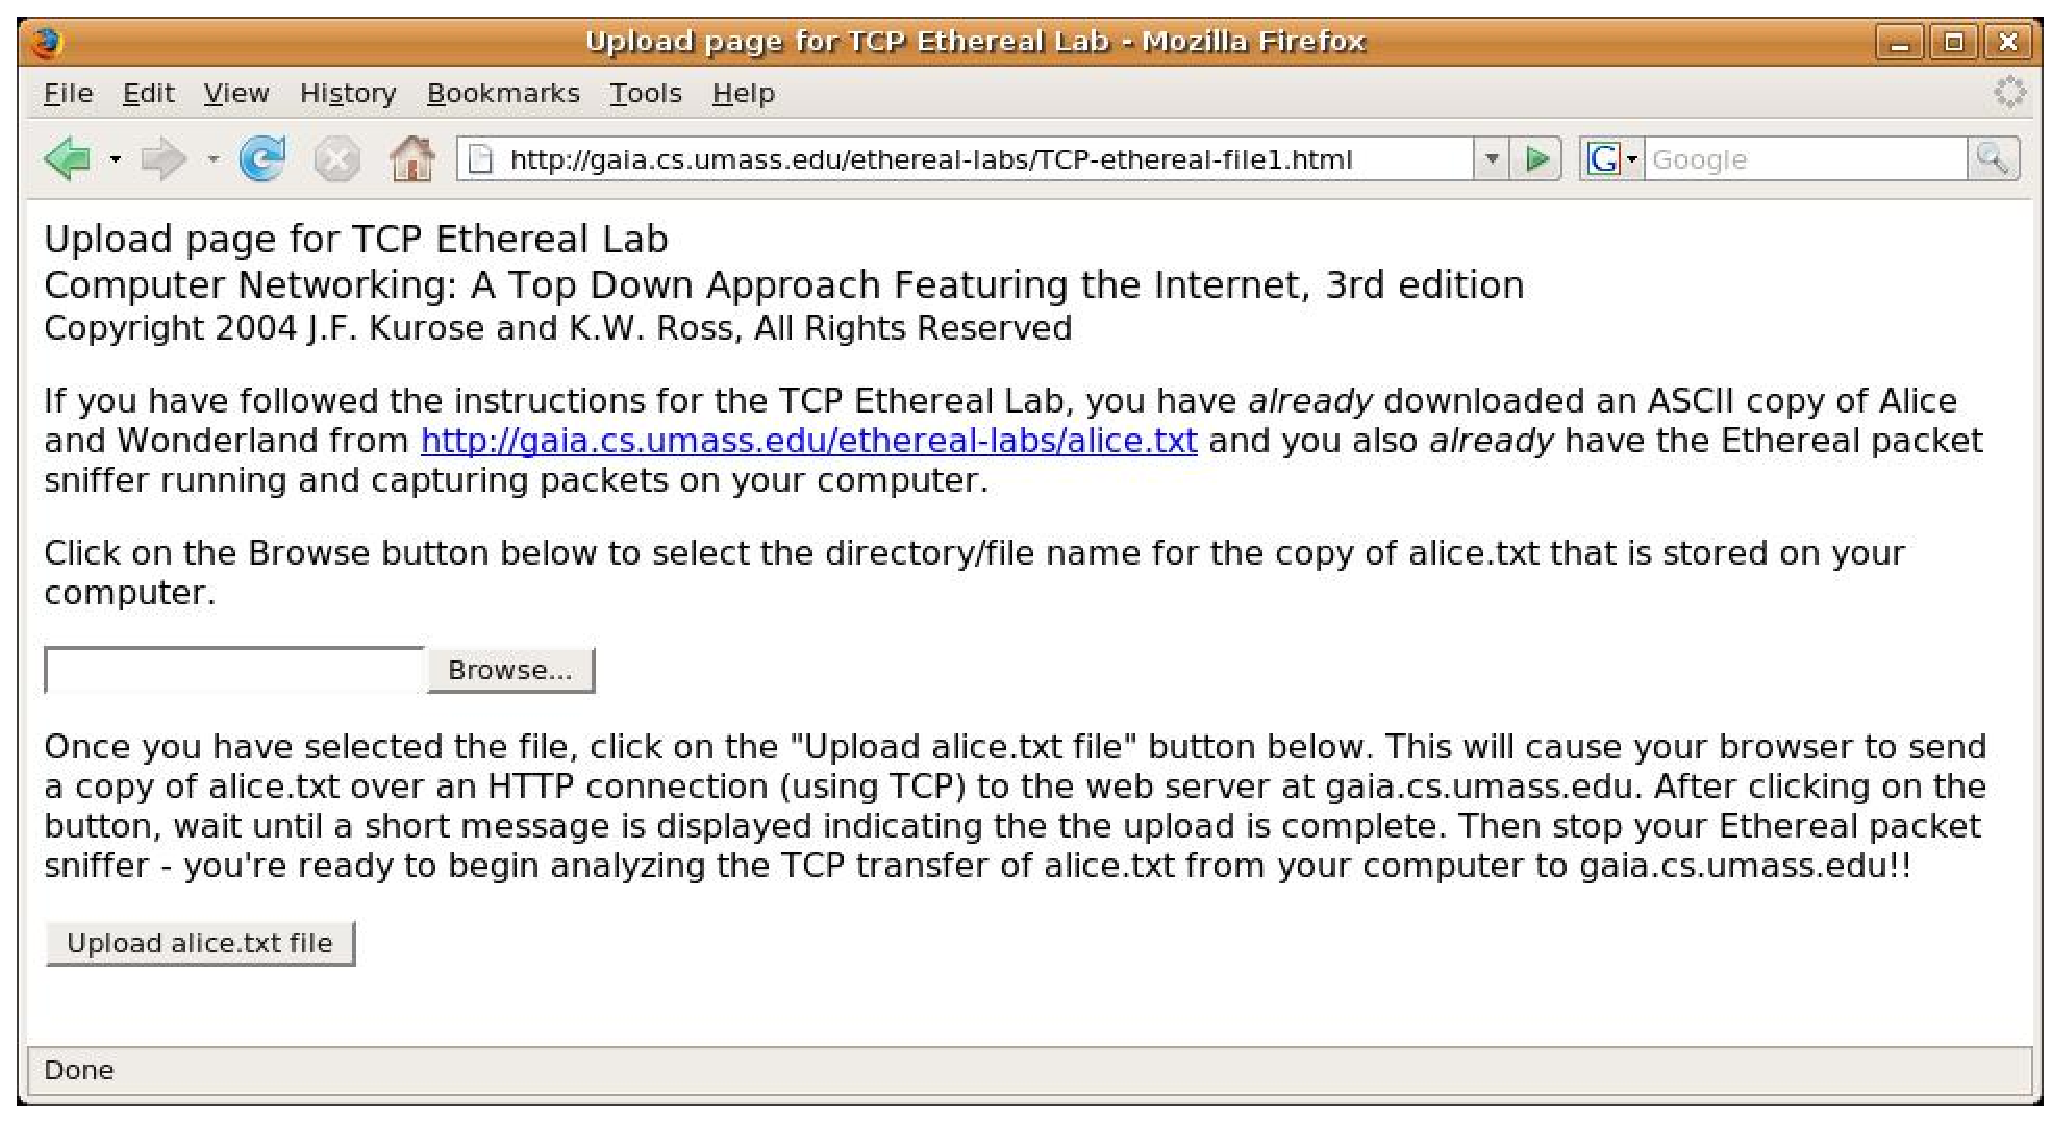
\includegraphics[width=0.99\columnwidth]{figs/lab_4_fig_1.eps}
    %\includegraphics[width=0.99\columnwidth]{lab_2_fig_1.jpg}
    \caption{Upload page}\label{lab_4_fig_1}
\end{figure}
\item Use the {\em Browse} button to enter the full
  path name of alice.txt on the client computer, and then press the
  {\em Upload alice.txt file} button to upload the file to the server
 \url{gaia.cs.umass.edu}.
\item Once the file has been uploaded, a new web page, which is a
  short congratulation, will be transferred from the Web server to the
  client and displayed in the web browser, as shown in Figure~\ref{lab_4_fig_2}.
\begin{figure}[ht]
    \centering
    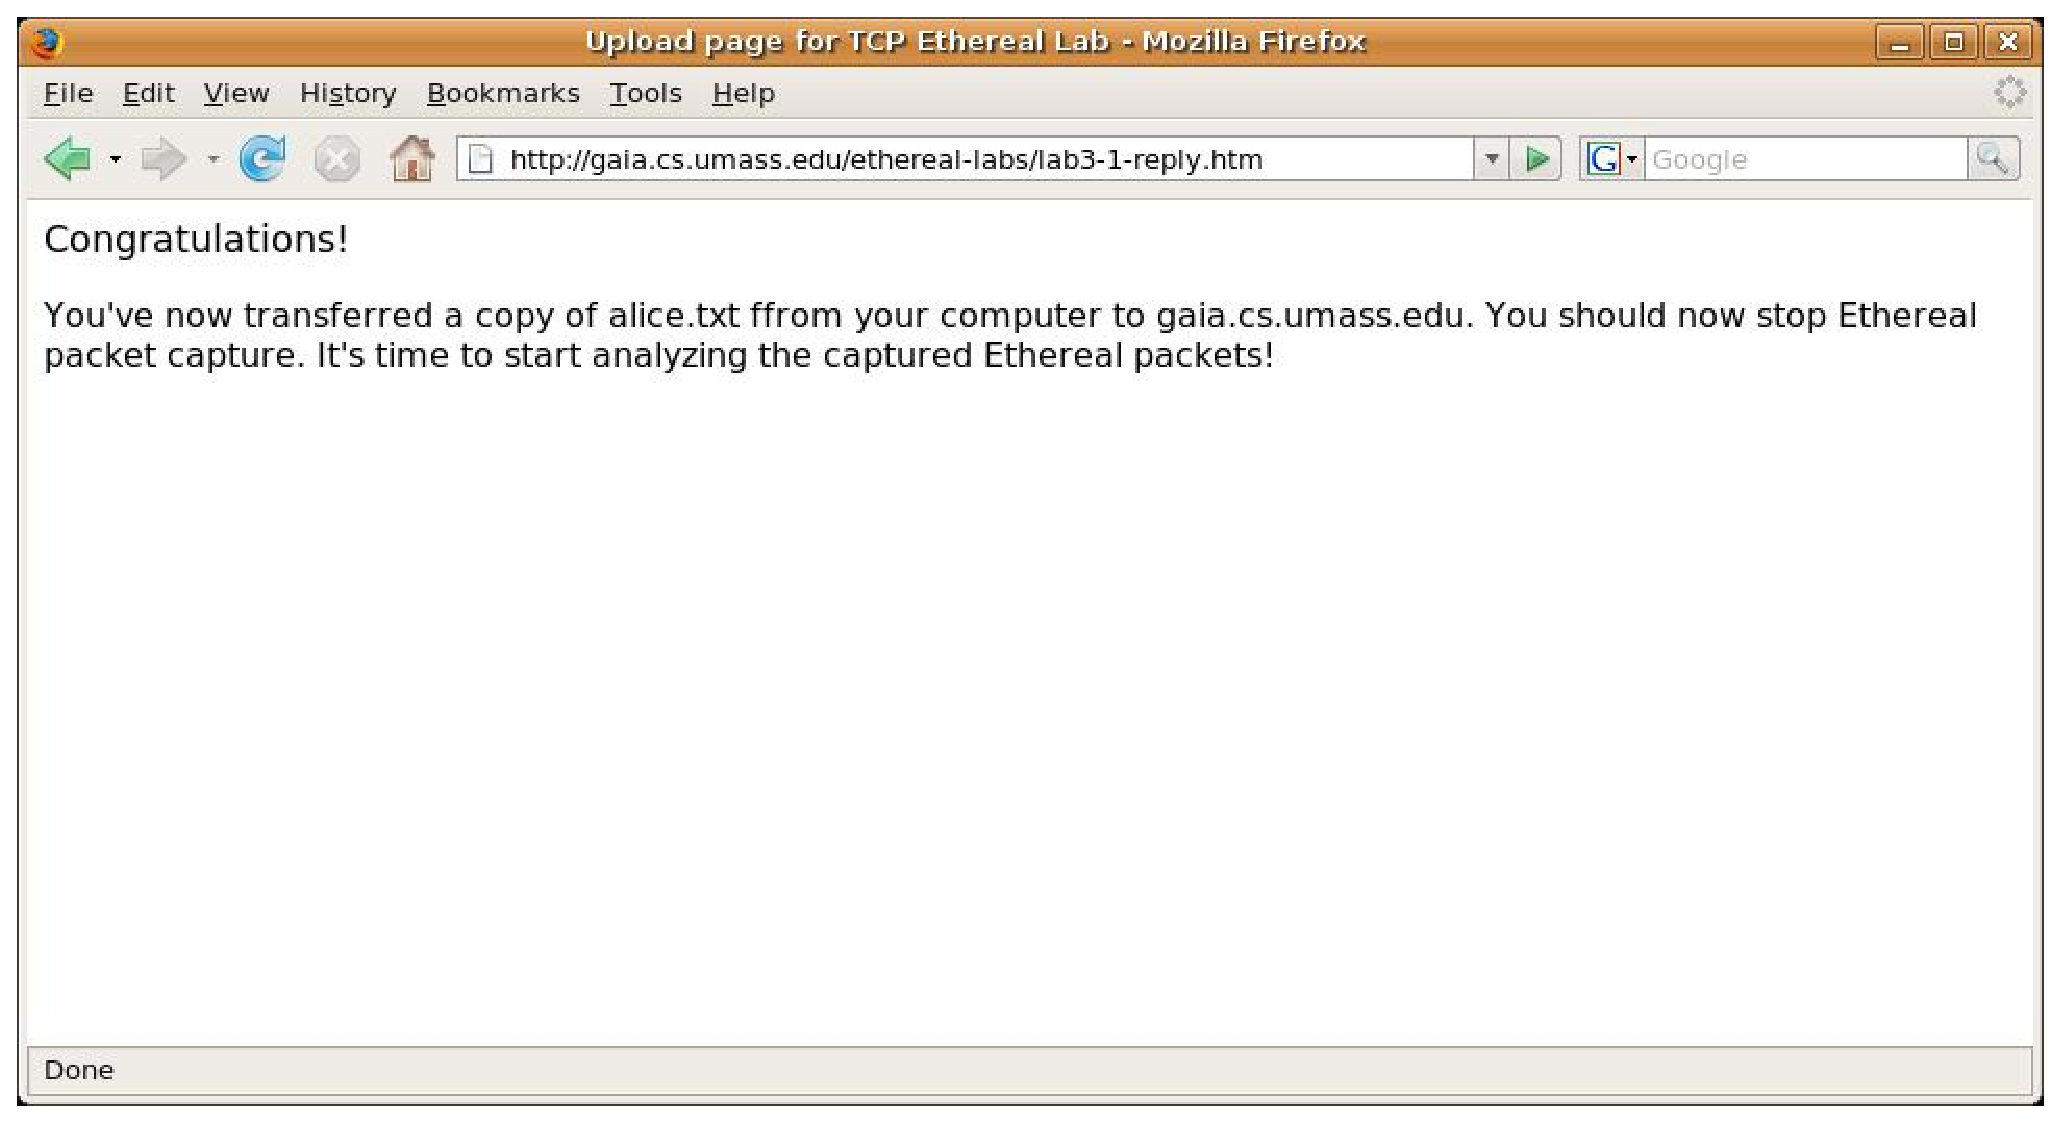
\includegraphics[width=0.99\columnwidth]{figs/lab_4_fig_2.eps}
    %\includegraphics[width=0.99\columnwidth]{lab_2_fig_2.jpg}
    \caption{Congratulation Page}\label{lab_4_fig_2}
\end{figure}
\end{itemize}

To transfer alice.txt and the congratulation page without
error, a TCP connection between the client and the server is
established.  The TCP connection completes the four operations in this
real-world application as follows:

\begin{itemize}
    \item TCP connection setup.
    \item Transfer the HTTP POST command and the file alice.txt, from
      the client computer to the server \url{gaia.cs.umass.edu}.
    \item Transfer the congratulation page from the server to the client.
    \item TCP connection release.
\end{itemize}

WireShark is run on the client computer to capture the trace of the
TCP segments sent/received from/to the client computer while the
file is being transferred. We saved the trace from the TCP stream in
the file {\bf tcp-trace-1.cap}. The trace tracked all of the above
four actions of TCP. We use this trace to study the 
TCP behaviours in this lab.

\subsection{TCP Header Format}

\hspace*{0.5cm} Every TCP segment consists of a header followed by an
optional data portion. The format of the header is defined in RFC 793,
including Source Port (16 bits), Destination Port (16 bits), Sequence
Number (32 bits), ACK (32 bits), .... In this lab, we will see the
details of the TCP headers used in this 
application.

\subsection{TCP Connection Setup}

\hspace*{0.5cm} Before transferring data, a TCP connection is
established between the two end systems, typically with  three messages,
called the three-way handshake: SYN $\rightarrow$ SYNACK $\rightarrow$
ACK.  The handshake is also used to negotiate certain properties of
the connection, e.g., the Maximum Segment Size (MSS) that the client
and server can accept, and the Selective Acknowledgement (SACK)
option.  In this lab, we will see the three-way handshake procedure in
the trace {\bf tcp-trace-1.cap}.%  The initial sequence number for
% each direction and some properties were set in the three-way
% handshake.

\subsection{TCP Data Flow}

\hspace*{0.5cm} Once the connection is established, the TCP sender
partitions the message from the application into segments. The MSS is
used to determine how to partition the single message so the
underlying network can encapsulate each segment into a packet without
further fragmentation.  The sequence number and ACK number are used to
detect packet loss, duplication, re-order in transmission and to
deliver the segments correctly and in-order to the application in the
destination host.

In this real-world application, after the connection was established,
the client computer wrote about 300KB into the data stream using
the HTTP POST command. From the application's perspective, this was
sent as one unit, or one message. However, the underlying network
cannot support packets large enough to hold all 300KB of
data. We will see that TCP broke this single logical transmission into
multiple segments according to MSS.

In the trace file {\bf tcp-trace-1.cap}, the first three segments are
used to establish the connection. Starting from the No.4 TCP segment,
the client  began to transfer the application layer message to
the server. The 4th segment contains the HTTP POST command (we will
dig into the packet content field and see this HTTP command).  This
segment is actually used to transfer this HTTP command. The text file
is transferred by the following TCP segments. Here we regard both the
HTTP POST command and the file (alice.txt) together as the whole
message. Therefore, we consider the 4th TCP segment as the first
segment in the TCP connection to transfer the message from the
client to the server.

\subsection{TCP Connection Release}

\hspace*{0.5cm} The TCP connection is closed when the two end systems
exchange TCP segments with FIN bit set and ACKed by the other side.
The FIN bit literally means that no additional new data will be sent
on that side of the connection.

The sequence of two FINs and their corresponding ACKs is the preferred
way to gracefully terminate a TCP connection. However, TCP connections
can also be terminated by setting the RESET bit.  Although the RESET
was designed to be used for unrecoverable errors, it is often used in
practice for fast termination that avoids the formalities of the
FIN-ACK exchanges.

In the trace file {\bf tcp-trace-1.cap}, after the client
acknowledged the data of the congratulation page, the server sent a
FIN indicating that it would not be sending any additional data. The
client acknowledged this FIN by sending back the ACK. Therefore the
flow in the direction from the serve to the client is closed. The
client computer could also terminate its flow to the server by
sending the FIN segments. Alternatively, the client computer 
sent a RESET segment to the server to release the connection.



\subsection{TCP Congestion Control (Optional)} 

\hspace*{0.5cm} In TCP, congestion control provides the ability to
limit the sending rate in response to signs of network congestion.
Congestion control helps the network to recover from congestion by
shrinking sender's outgoing traffic and therefore avoids network
congestion collapse, and at the same time tries to achieve
throughput as high as possible.

Congestion control is realized by setting the size of congestion
window, according to two strategies, the slow start and the congestion
avoidance. During the slow start phase, the congestion window increases 
one MSS with each acknowledgement, and subsequently 
the window size is doubled every round-trip time (RTT). During congestion
avoidance, each acknowledgement increases the congestion window by
$MSS^2/ congestion\ window\ size$ (if the receiver sends ACK for each
received packet without delay), and subsequently the congestion window
size is increased by one MSS every RTT. Slow start phase changes to
congestion avoidance phase when congestion window exceeds the
slow-start threshold.

We will use the TCP segment trace file,
\textbf{tcp-trace-1.cap} to
investigate TCP congestion control. In particular, we 
look at how the congestion window evolved since the beginning of
transferring the HTTP POST command and the alice.txt file.

\subsection{TCP Flow Control (Optional)}

\hspace*{0.5cm} TCP also provides flow control or the ability to limit
the sending rate to avoid a fast
sender over-running a slow receiver. To provide a reliable service,
a TCP receiver cannot deliver data that it received out of order to
the waiting application. Therefore, the TCP receiver typically
allocates a fixed amount of buffer space to store both out-of-order
data and data waiting for the application to fetch. If the TCP
receiver runs out of buffer space to hold the incoming data, then it
has no choice but to drop the out-of-order data packet even
if it is error-free.

The receiver advertises its available buffer in each acknowledgement.
The receiver's advertised window field is used to inform the sender
how much room is left for the incoming data. Then in the sliding-window
based flow control, the sender chooses the minimum of the receiver
window and the congestion window to be the size of the sliding window in
order to make sure that the receiver will not run out of buffer
space.

In this subsection, we will still use the TCP segment trace file,
\textbf{tcp-trace-1.cap}, to exam TCP flow control. We will see that
the receiver window took effect and throttled the sender even though
the congestion window continued to grow.

\subsection{Retransmission in TCP}

\hspace*{0.5cm} We learned that TCP provides reliable data
transmission over an unreliable network by relying on feedback from
the receiver to detect loss and responding to packet loss with
retransmissions. TCP uses two kinds of indications of packet losses,
time-out and duplicated acknowledgement (which is regarded as an early
indication of packet loss and causes the fast retransmission instead
of waiting until timeout). The TCP sender must maintain a copy of the
data it sent in case retransmission is needed, so it must store the
data until the corresponding acknowledgement is received.

However, in the trace \textbf{tcp-trace-1.cap}, all the packets were
received correctly the first time and thus there was no
retransmission. In order to investigate the TCP retransmission
scheme, we are going to analyse another trace of TCP connections,
\textbf{tcp-trace-retransmission.cap}~\cite{Matthews04}, in which
retransmission does occur.

The trace, \textbf{tcp-trace-retransmission.cap}, was taken on a
private network~\cite{Matthews04}. A desktop PC and a laptop were
connected via a wireless router. The laptop was connected via a
wireless interface and specifically placed so as to interfere with a
strong signal. The IP addresses of the desktop and the laptop are,
respectively, 192.168.0.100 and 192.168.0.102. The desktop sent a file
(about 40K bytes) to the laptop using TCP. The TCP port number for the
desktop is 4480, and 5001 for the laptop. The experiment configuration
is shown in Figure~\ref{lab_4_fig_config}. WireShark was run on the sender,
i.e., the desktop, while the file was being transferred to capture the
TCP segments exchanged. The TCP connection trace was saved in file
\textbf{tcp-trace-retransmission.cap}.

\begin{figure}[ht]
    \centering
    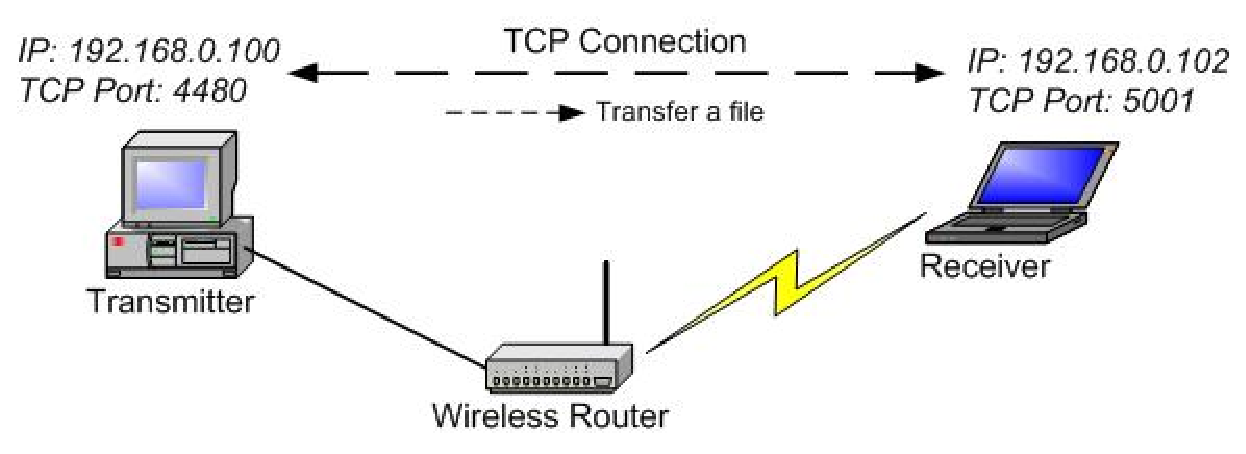
\includegraphics[width=0.99\columnwidth]{figs/lab_4_network_configuration.eps}
    %\includegraphics[width=0.99\columnwidth]{lab_2_fig_1.jpg}
    \caption{Network Configuration}\label{lab_4_fig_config}
\end{figure}

In this lab, we will take a look at both the fast retransmission and
the time out retransmission using this trace file.

\section{Procedures}

{\bf Note:}  You will answer a set of questions by exploring the 
trace file {\bf tcp-trace-1.cap} and {\bf tcp.analysis.retransmission.cap}.
 Whenever possible, when answering a 
question you should provide the information of the packet(s) within 
the trace that you used to answer the question asked. The information 
includes the Packet No., the name(s) and value(s) of the packet field(s) 
that you use to answer the questions.

\subsection{TCP Header Format}
\begin{itemize}
\item Download the traces folder from the lab website.

\item Open the captured trace file named {\bf tcp-trace-1.cap} with
  WireShark.  Now what you should see is a series of TCP segments sent
  between the client  and the server \url{gaia.cs.umass.edu}.

\item Since this lab is about TCP rather than HTTP, change WireShark's
  {\em Packet List Pane} window so that it shows information about the
  TCP segments containing the HTTP messages.
  % , rather than about the HTTP messages.
  To do this, in WireShark, select {\em Analyze $\Rightarrow$ Enabled
    Protocols}. Then uncheck the {\em HTTP box} and select {\em OK}.
\item Select the first packet and explore the details of the TCP
  segment using the {\em packet details pane} and the {\em packet bytes
  pane}.
\item Select the {\em Transmission Control Protocol} item in the
  \emph{Packet Details Pane} then the content of the header is
  highlighted in the {\em Packet Bytes Pane}.
  % port 80 => Hex 0050, 4335 => Hex 10ef
\item Answer the related questions in section \ref{sec:tcp-head}.

\end{itemize}

\subsection{TCP Connection Setup}

\begin{itemize}
\item Find the initial three-way handshake in the trace file. (Hint: 
  You should see the SYN segment sent from the client to 
  \url{gaia.cs.umass.edu}, and also the SYNACK segment being returned.)
\item Answer the related questions in section \ref{sec:tcp-con}.
\end{itemize}

\subsection{TCP Data Flow}

\begin{itemize}
\item Check the HTTP POST command. Select the 4th segment in the {\em
    Packet List Pane}. Select the {\em Data} item in the {\em Packet
    Details Pane} and the content of the data carried by this segment
  is highlighted in the {\em Packet Bytes Pane}. You should find a
  POST and other HTTP command information within its {\em Date} field.

\item Set time reference. In order to make the following analysis
  easier, set time reference to the 4th packet. Choose the {\em Time
    Reference} items in the {\em Edit} menu, or from the pop-up menu
  of the {\em Packet List Pane}.

  {\bf Note:} Now the 4th packet becomes the starting point for all
  subsequent packets. The time values of all the following packets are
  calculated relative to this packet.

\item Set the time display format as microseconds. Choose the {\em
    Time Display Format} in the {\em View} menu. Then select {\em
    Seconds Since Beginning of Capture} and {\em Microseconds}.

\item Answer the related questions in section \ref{sec:2.4.3}.
\end{itemize}

\subsection{TCP Connection Release}

\begin{itemize}
\item Find the segments used to release the connection between the 
client and the server.
\item Answer the related questions in section \ref{sec:2.4.4}.
\end{itemize}



\subsection{TCP Congestion Control}\label{sec:3.3.1}

\begin{itemize}
  \item Download the HTTP traces folder from the lab website.
  \item Open the captured trace file named \textbf{tcp-trace-1.cap}
    with WireShark.
  \item Since this lab is about TCP rather than HTTP, change
    WireShark's {\em Packet List Pane} window so that it shows
    information about the TCP segments containing the HTTP messages.
    To do this, select {\em Analyze $\Rightarrow$ Enabled Protocols}.
    Then uncheck the {\em HTTP box} and select {\em OK}.
  \item Set time reference. In order to make the following analysis
    easier, set time reference to the 4th packet. Choose the {\em Time
      Reference} items in the {\em Edit} menu, or from the pop-up menu
    of the {\em Packet List Pane}.
  \item Answer the related questions in section \ref{sec:3.4.1}.
\end{itemize}

\subsection{TCP Flow Control}\label{sec:3.3.2}

\begin{itemize}
\item Open the captured trace file named {\bf tcp-trace-1.cap} with
  WireShark.
\item Answer the related questions in section \ref{sec:3.4.2}.
\end{itemize}

\subsection{Retransmission in TCP (Optional)}\label{sec:3.3.3}

\begin{itemize}
\item Open the captured trace file named
  \textbf{tcp-trace-retransmission.cap} with WireShark.
\item List retransmissions. Search for retransmissions with the
  display filter \emph{tcp.analysis.retransmission}. Applying this
  filter, you should see 9 retransmissions in the trace.
\item Answer the related questions in section \ref{sec:3.4.3}.
\end{itemize}

\section{Discussion}

\subsection{TCP Header Format}\label{sec:tcp-head}

\begin{enumerate}
\item Write down the TCP header content in hexadecimal format (in the
  {\em packet bytes pane}). Dissect the TCP header and indicate the
  value of each field in the header. Annotate the
  hexadecimal content to explain your answer.
\item What are TCP port numbers used by the client computer (source)
  and the server (destination) when transferring the file to
  \url{gaia.cs.umass.edu}? How did the client computer determine the
  port numbers when it wanted to set up a TCP connection to the
  server?
\item What is the maximum header length? Given the value of the Header
  Length field, how to calculate the length of the head in unit of
  bytes? Verify your answer using the first TCP segment in the trace
  file.
\item (Optional) How does TCP calculate the Checksum field? What is
  the pseudo-header format? Write down the pseudo-header of the flow
  from the client to the server in hexadecimal format. Verify the
  Checksum value in the first TCP segment in the trace file.
% c: too time-consuming
\end{enumerate}

\subsection{TCP Connection Setup} \label{sec:tcp-con}
\begin{enumerate}
\item Which segments are the initial three-way handshake in the trace
  file? How do you determine this?
\item What is the actual initial sequence number in each direction (in
  hexadecimal format)? How did the client  and the server
  determine these values?

  {\bf Note:} WireShark displays the relative sequence number. You
  should select the {\em Sequence Number} field in the header, the
  actual value is highlighted in the {\em Packet Bytes Pane}.

\item What is the value of the acknowledgement number in the SYNACK
  segment? How did \url{gaia.cs.umass.edu} determine that value?

\item What are the values of the sequence number and the
  acknowledgement number in the third ACK segments in the three-way
  handshake? How did the client computer determine these values?

\item How did the client and the server announce the maximum
  TCP payload size that they were willing to accept? What are the
  values and why did they choose these values?

\item Is there data sent in the SYN, SYNACK, and ACK segment? How do
  you determine this?
\end{enumerate}

\subsection{TCP Data Flow}\label{sec:2.4.3}
\begin{enumerate}
\item Beginning with the 4th segment, what are the sequence number,
  acknowledgement number, data length, and the time of the segment
  sent/received from/to the client computer of the 4th, 5th, 6th, ...,
  15th segments in the TCP connection? Fill out Table~\ref{lab_2_tab_1} for the data
  flow from the client computer to the server. ({\bf Note:} list both the actual
  value and relative value of the sequence number and acknowledgement
  number.)
\begin{table}[ht]
    \centering
    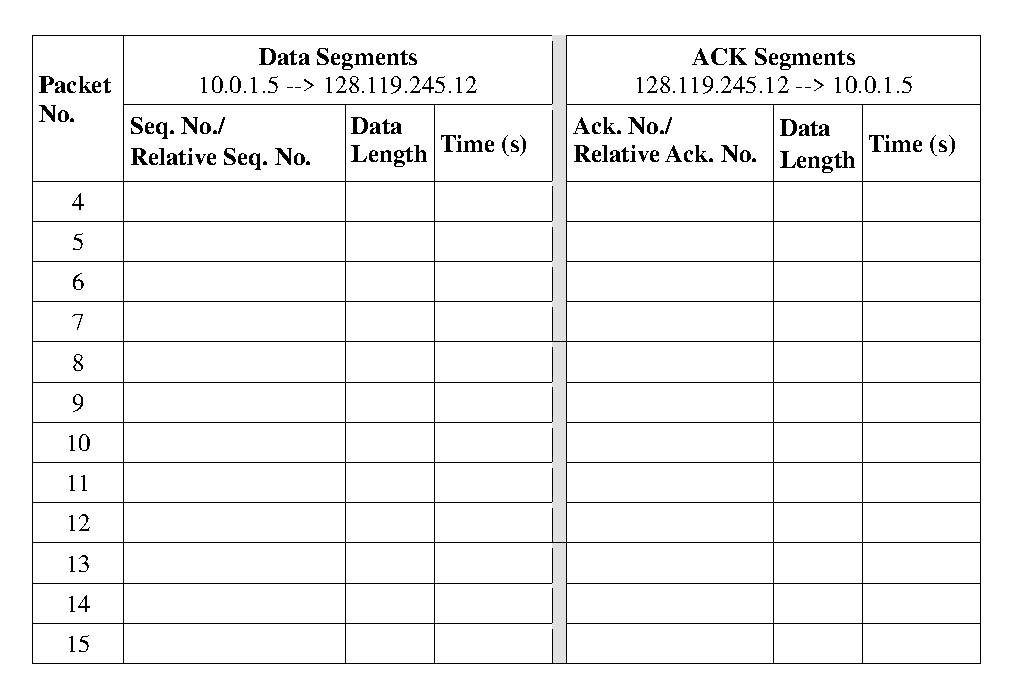
\includegraphics[width=0.75\columnwidth]{figs/lab_4_table_1.eps}
    %\includegraphics[width=0.99\columnwidth]{lab_2_fig_1.jpg}
    \caption{TCP segment exchange table (Please show the segment and its acknowledgement in the same row.)}\label{lab_2_tab_1}
\end{table}

\item What are the segments acknowledged by the packet 6, 9, 12, and
  15, respectively? ({\bf Hint:} acknowledgement number is the next
  byte expected, so it actually acknowledges the bytes before the
  acknowledgement number.)

\item Given the difference between when each TCP segment was sent, and
  when its acknowledgement was received, what is the RTT value for each
  of the segments which have been acknowledged before the 15th
  segment?

\item (Optional) What is the Estimated RTT value after the receipt of
  each ACK?  Assume that the value of the Estimated RTT is equal to
  the measured RTT for the first segment, and then is computed using
  the Estimated RTT equation for all subsequent segments.  ({\bf
    Hint:} Compare your calculation with the statistics analysis of
  TCP stream by WireShark.  See Section 3.5).

%WireShark also has a nice feature that allows you to plot the RTT
%for each of the TCP segments sent. Select a TCP segment in the
%packet list pane that is being sent from the client to the
%gaia.cs.umass.edu server. Then select: {\em Statistics->TCP Stream
%Graph->Round Trip Time Graph}.)

\item In the trace file, how did the sequence number of the packets 
  from the server to the client change? Why? (\textbf{Hint}: 
  When transferring the alice.txt file, the server was only a receiver 
  and did not send any data to the client.)

\item (Optional) At the end of the trace file, find the TCP segments used by the
  server to transfer the congratulation web page to the client
  computer? How do you determine this?

%\item What is the minimum amount of available receiver buffer space
%  advertised by the receiver for the entire trace? Did the lack of
%  receiver buffer space ever throttle the sender?

\item (Optional) Are there any retransmitted segments in the trace
  file? What do you check for (in the trace) in order to answer this
  question?

% \item How much data did the receiver typically acknowledge in an ACK?
%   Can you identify cases where the receiver was ACKing every other
%   received segment?

% \item Find some TCP segments in which the PSH bit is set. What is the
%   length of these segments? What is the PSH bit used for these TCP
%   segments?
\end{enumerate}

\subsection{TCP Connection Release}\label{sec:2.4.4}
\begin{enumerate}
\item Which packets were used to close the data flow from the server
  to the client? How do you determine this? ({\bf Hint:} two segments
  are involved in the FIN-ACK sequence.)
\item Which packets were used to close the data flow from the client
  to the server? How do you determine this?
\item (Optional) In the FIN segment, what is the sequence number? In the
  corresponding ACK segment, what is the acknowledgement number? How
  did the client determine this number?
\end{enumerate}




\subsection{TCP Congestion Control} \label{sec:3.4.1}

\begin{enumerate}
\item Exam the 4th to 15th TCP segments and take a reference to
  the Table in Question 1 of Section \ref{sec:2.4.3} in Lab 2. Can you
%c: set \label{sec:2.4.3} to the corresponding section in Lab 2.
  find a pattern of the number of segments sent from the client
  and from the server \url{gaia.cs.umass.edu}? Why did the
  TCP data flow have such a pattern?

\item What is the initial size of congestion window? How do you
  determine this? What is the size of congestion window when the
  segment 5, 8, 11 and 14 were sent out?

\item In the lecture we have learned that the congestion window
  doubles its size in every RTT in the slow start phase. Beginning
  with the 4th packet, what is the size of the congestion window and
  which packet were inside the congestion window (i.e., these packets
  could be sent) during the first RTT? What is the size of the
  congestion window and which packet were inside the congestion window
  during the second RTT? How about the third RTT? Give the segment
  numbers.

\item When did the sender's congestion control change from the slow
  start phase to the congestion avoidance phase? Give the segment
  number and the time. How do you determine this?

% \item What is the pattern of exchanging TCP segments between the
%   client and the server in congestion avoidance phase? Give the
%   numbers of some TCP segments sent by the client during congestion
%   avoidance phase.
% c: redundant

\item What is the threshold between the slow start and congestion
  avoidance? (\textbf{Hint:} the size of congestion window when TCP
  change from slow start phase to congestion avoidance phase.)
\end{enumerate}

\subsection{TCP Flow Control}\label{sec:3.4.2}

\begin{enumerate}
\item Exam the 179th segment in the trace file, why did the sender
  stop sending more segments? What is the size of receiver window
  advertised by the receiver at this moment? How do you determine
  this?
\end{enumerate}

\subsection{Retransmission in TCP (Optional)}\label{sec:3.4.3}

\begin{enumerate}
\item Segment 12 is the first retransmission. What is it in the
  segment that identifies the segment as a retransmission? (Hint: the
  sequence number has been used by a previous packet.) Which segment
  was segment 12 retransmitted for?

\item Segment 12 is a fast retransmission, which should be triggered
  by triple-duplicated-acknowledgment. Find the three acknowledgments
  which triggered the fast retransmission of segment12. (Hint: in
  order to trigger a fast retransmission, the duplicated
  acknowledgments should acknowledge the same acknowledgment number,
  which is the sequence number of the fast retransmission.)

\item Is segment 44 a fast retransmission or timeout retransmission?
  How do you determine this? (Hint: whether the sequence number in the
  segment has been acknowledged for three times or not.)

% \item Which segment(s) did segment 44 retransmit for? What is the
%   timeout duration, i.e. the time interval between the original
%   segment and its retransmission? Compare the timeout duration with
%   RTT. It this timeout duration reasonable? You have got the Estimated 
%   RTT in Question 4 in Section~\ref{sec:2.4.3}.
% c: too time-consuming
\end{enumerate}